\documentclass[12pt,twoside,letterpaper]{article}
%NOTE: This report format is 
\setlength{\footskip}{1.5cm}

\newcommand{\reporttitle}{Procesadores de Lenguajes: Memoria del Proyecto}
\newcommand{\reportauthorOne}{Jose Luis Prado Sierra}
\newcommand{\cidOne}{220070}
\newcommand{\reportauthorTwo}{Alejandro Gragera Serradilla}
\newcommand{\cidTwo}{22M043}
\newcommand{\reportauthorThree}{Antonio Bielza Díez}
\newcommand{\cidThree}{22M049}
\newcommand{\reporttype}{Coursework}
\bibliographystyle{plain}

% include files that load packages and define macros
\input{includes} % various packages needed for maths etc.
\input{notation} % short-hand notation and macros


%%%%%%%%%%%%%%%%%%%%%%%%%%%%

\begin{document}
% front page
% Last modification: 2016-09-29 (Marc Deisenroth)
% Modification for UW: 2017-05-22 (jphickey)
\begin{titlepage}

\newcommand{\HRule}{\rule{\linewidth}{0.5mm}} % Defines a new command for the horizontal lines, change thickness here


%----------------------------------------------------------------------------------------
%	LOGO SECTION
%----------------------------------------------------------------------------------------



\begin{center} % Center remainder of the page

%----------------------------------------------------------------------------------------
%	HEADING SECTIONS
%----------------------------------------------------------------------------------------

\includegraphics[width = 9cm]{./figures/etsiinf}\\[1.5cm] 
%\textbf{\textsc{\Large Procesadores de Lenguajes}}\\[1.0cm] 
\textsc{\Large Universidad Politécnica de Madrid}\\[0.5cm] 

%----------------------------------------------------------------------------------------
%	TITLE SECTION
%----------------------------------------------------------------------------------------
\vspace{0.75cm}
\HRule \\[0.4cm]
{ \huge \bfseries \reporttitle}\\ % Title of your document
\HRule \\[0.7cm]
    \textsc{\large Analizador Léxico y Tabla de Símbolos}
\end{center}
%----------------------------------------------------------------------------------------
%	AUTHOR SECTION
%----------------------------------------------------------------------------------------

%\begin{minipage}{0.4\hsize}
\vfill
\begin{flushright} \large
    \textsc{\textbf{Grupo 18}}
\\
\reportauthorOne - \cidOne\\ % Your name
\reportauthorTwo - \cidTwo\\ % Your name
\reportauthorThree - \cidThree\\ % Your name
\end{flushright}
%\vspace{4cm}
%\makeatletter
%Date: \@date 

%\vfill % Fill the rest of the page with whitespace



\makeatother


\end{titlepage}




%%%%%%%%%%%%%%%%%%%%%%%%%%% table of content
%If a table of content is needed, simply uncomment the following lines
%\tableofcontents
%\newpage

%%%%%%%%%%%%%%%%%%%%%%%%%%%% Main document
%\section*{Note:}
%\emph{This document is intended to provide a sample structure for the reports in ME303 at the University of Waterloo. }

\section{Analizador Léxico}
%\emph{Describe the physical problem under investigation and the briefly summarize the governing equations. Example:}

Durante el desarrollo del Analizador Léxico hemos descrito una serie de objetos y estructuras matemáticas indispensables para que su diseño, desarrollo y función final cumplan con las expectativas de un Procesador de Lenguajes.

\subsection{Tokens}

Los tokens son duplas que se generan cuando el Analizador Léxico encuentra una concatenación de caracteres que identifica como válida. 
\\
Contienen la información necesaria para que las reciba el Analizador Sintáctico y se componen de un código que los identifica y un atributo opcional que puede servir para diferenciarlos de otros tokens con el mismo código o aportar información extra.
\\
\\
Hemos definido los siguientes tokens en funcion de las necesidades de nuestra práctica:

\begin{itemize}[itemsep=0.1em, topsep=1em, parsep=0pt, partopsep=0pt]
    \item Boolean: $<$BOOLEAN, $>$
    \item Else: $<$ELSE, $>$
    \item Float: $<$FLOAT, $>$
    \item Function: $<$FUNCTION, $>$
    \item If: $<$IF, $>$
    \item Int: $<$INT, $>$
    \item Let: $<$LET, $>$
    \item Read: $<$READ, $>$
    \item Return: $<$RETURN, $>$
    \item String: $<$STRING, $>$
    \item Void: $<$VOID, $>$
    \item Write: $<$WRITE, $>$
    \item Constante real: $<$REALCONST, $>$
    \item Constante entera: $<$INTCONST, $>$
    \item Cadena: $<$STR, "c*"$>$
    \item Identificador: $<$ID, posTS$>$
    \item Suma con asignación (+=): $<$PLUSEQ, $>$
    \item Igual (=): $<$EQ, $>$
    \item Coma (,): $<$COMMA, $>$
    \item Punto y coma (;): $<$SEMICOLON, $>$
    \item Paréntesis abierto ((): $<$OPPAR, $>$
    \item Paréntesis cerrado ()): $<$CLPAR, $>$
    \item Llave abierta (\{): $<$OPBRA, $>$
    \item Llave cerrada (\}:) $<$CLBRA, $>$
    \item Suma (+): $<$SUM, $>$
    \item Y Lógico (\&\&): $<$AND, $>$
    \item Menor ($<$): <MINORTHAN, $>$
    \item false: $<$FALSE, $>$
    \item true: $<$TRUE, $>$
    \item EOF: $<$EOF, $>$
\end{itemize}

Todos los tokens definidos conforman la parte común, específica y opcional de los requeridos.


\begin{center}
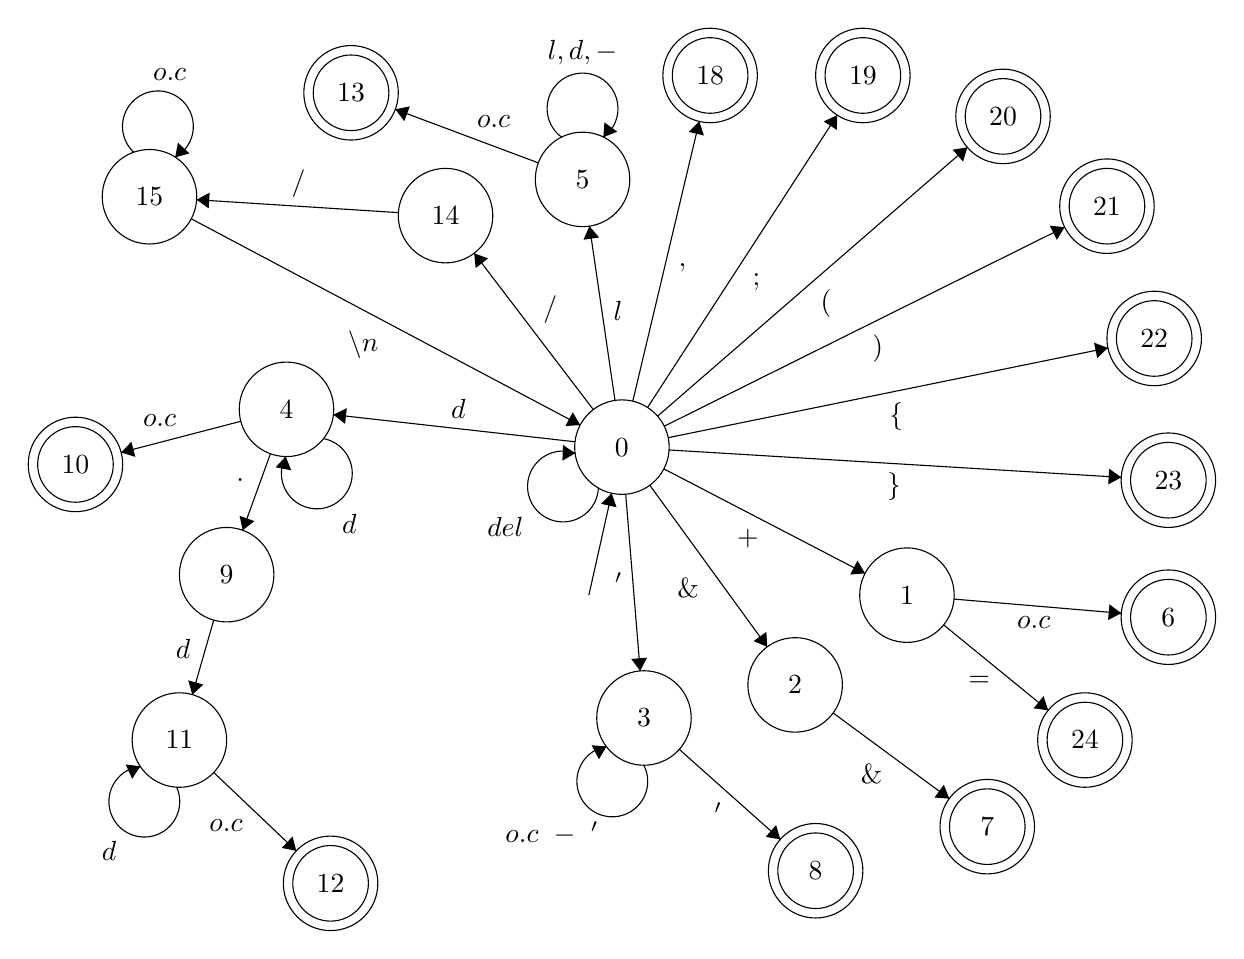
\begin{tikzpicture}[scale=0.2]
\tikzstyle{every node}+=[inner sep=0pt]
\draw [black] (39.8,-27.7) circle (3);
\draw (39.8,-27.7) node {$0$};
\draw [black] (57.9,-37.1) circle (3);
\draw (57.9,-37.1) node {$1$};
\draw [black] (74.5,-38.5) circle (3);
\draw (74.5,-38.5) node {$6$};
\draw [black] (74.5,-38.5) circle (2.4);
\draw [black] (69.2,-46.3) circle (3);
\draw (69.2,-46.3) node {$24$};
\draw [black] (69.2,-46.3) circle (2.4);
\draw [black] (50.8,-42.8) circle (3);
\draw (50.8,-42.8) node {$2$};
\draw [black] (63,-51.8) circle (3);
\draw (63,-51.8) node {$7$};
\draw [black] (63,-51.8) circle (2.4);
\draw [black] (41.2,-44.9) circle (3);
\draw (41.2,-44.9) node {$3$};
\draw [black] (52.1,-54.6) circle (3);
\draw (52.1,-54.6) node {$8$};
\draw [black] (52.1,-54.6) circle (2.4);
\draw [black] (18.5,-25.3) circle (3);
\draw (18.5,-25.3) node {$4$};
\draw [black] (5.1,-28.8) circle (3);
\draw (5.1,-28.8) node {$10$};
\draw [black] (5.1,-28.8) circle (2.4);
\draw [black] (14.7,-35.8) circle (3);
\draw (14.7,-35.8) node {$9$};
\draw [black] (11.7,-46.3) circle (3);
\draw (11.7,-46.3) node {$11$};
\draw [black] (21.3,-55.4) circle (3);
\draw (21.3,-55.4) node {$12$};
\draw [black] (21.3,-55.4) circle (2.4);
\draw [black] (28.6,-13) circle (3);
\draw (28.6,-13) node {$14$};
\draw [black] (9.8,-11.8) circle (3);
\draw (9.8,-11.8) node {$15$};
\draw [black] (37.3,-10.7) circle (3);
\draw (37.3,-10.7) node {$5$};
\draw [black] (22.6,-5.2) circle (3);
\draw (22.6,-5.2) node {$13$};
\draw [black] (22.6,-5.2) circle (2.4);
\draw [black] (45.4,-4.1) circle (3);
\draw (45.4,-4.1) node {$18$};
\draw [black] (45.4,-4.1) circle (2.4);
\draw [black] (55.1,-4.1) circle (3);
\draw (55.1,-4.1) node {$19$};
\draw [black] (55.1,-4.1) circle (2.4);
\draw [black] (64,-6.7) circle (3);
\draw (64,-6.7) node {$20$};
\draw [black] (64,-6.7) circle (2.4);
\draw [black] (70.6,-12.4) circle (3);
\draw (70.6,-12.4) node {$21$};
\draw [black] (70.6,-12.4) circle (2.4);
\draw [black] (73.6,-20.8) circle (3);
\draw (73.6,-20.8) node {$22$};
\draw [black] (73.6,-20.8) circle (2.4);
\draw [black] (74.5,-29.8) circle (3);
\draw (74.5,-29.8) node {$23$};
\draw [black] (74.5,-29.8) circle (2.4);
\draw [black] (38.305,-30.288) arc (-2.28448:-290.28448:2.25);
\draw (33.58,-32.78) node [left] {$del$};
\fill [black] (36.84,-28.09) -- (36.06,-27.56) -- (36.02,-28.56);
\draw [black] (42.46,-29.08) -- (55.24,-35.72);
\fill [black] (55.24,-35.72) -- (54.76,-34.9) -- (54.3,-35.79);
\draw (47.8,-32.9) node [below] {$+$};
\draw [black] (60.23,-38.99) -- (66.87,-44.41);
\fill [black] (66.87,-44.41) -- (66.57,-43.51) -- (65.94,-44.29);
\draw (62.48,-42.19) node [below] {$=$};
\draw [black] (60.89,-37.35) -- (71.51,-38.25);
\fill [black] (71.51,-38.25) -- (70.76,-37.68) -- (70.67,-38.68);
\draw (65.95,-38.43) node [below] {$o.c$};
\draw [black] (41.57,-30.12) -- (49.03,-40.38);
\fill [black] (49.03,-40.38) -- (48.97,-39.43) -- (48.16,-40.02);
\draw (44.72,-36.63) node [left] {$\&$};
\draw [black] (53.21,-44.58) -- (60.59,-50.02);
\fill [black] (60.59,-50.02) -- (60.24,-49.14) -- (59.65,-49.95);
\draw (55.65,-47.8) node [below] {$\&$};
\draw [black] (40.04,-30.69) -- (40.96,-41.91);
\fill [black] (40.96,-41.91) -- (41.39,-41.07) -- (40.39,-41.15);
\draw (39.88,-36.36) node [left] {$'$};
\draw [black] (41.184,-47.888) arc (27.43495:-260.56505:2.25);
\draw (35.36,-51.45) node [below] {$o.c\mbox{ }-\mbox{ }'$};
\fill [black] (38.82,-46.71) -- (37.88,-46.63) -- (38.34,-47.52);
\draw [black] (43.44,-46.89) -- (49.86,-52.61);
\fill [black] (49.86,-52.61) -- (49.59,-51.7) -- (48.93,-52.45);
\draw (45.92,-50.24) node [below] {$'$};
\draw [black] (36.82,-27.36) -- (21.48,-25.64);
\fill [black] (21.48,-25.64) -- (22.22,-26.22) -- (22.33,-25.23);
\draw (29.41,-25.9) node [above] {$d$};
\draw [black] (20.842,-27.156) arc (79.34618:-208.65382:2.25);
\draw (22.49,-31.91) node [below] {$d$};
\fill [black] (18.45,-28.29) -- (17.81,-28.98) -- (18.8,-29.17);
\draw [black] (15.6,-26.06) -- (8,-28.04);
\fill [black] (8,-28.04) -- (8.9,-28.32) -- (8.65,-27.36);
\draw (10.44,-26.43) node [above] {$o.c$};
\draw [black] (17.48,-28.12) -- (15.72,-32.98);
\fill [black] (15.72,-32.98) -- (16.46,-32.4) -- (15.52,-32.06);
\draw (15.84,-29.77) node [left] {$.$};
\draw [black] (13.88,-38.68) -- (12.52,-43.42);
\fill [black] (12.52,-43.42) -- (13.22,-42.78) -- (12.26,-42.51);
\draw (12.43,-40.49) node [left] {$d$};
\draw [black] (11.522,-49.283) arc (24.30891:-263.69109:2.25);
\draw (7.24,-52.67) node [below] {$d$};
\fill [black] (9.22,-47.97) -- (8.29,-47.85) -- (8.7,-48.76);
\draw [black] (13.88,-48.36) -- (19.12,-53.34);
\fill [black] (19.12,-53.34) -- (18.89,-52.42) -- (18.2,-53.15);
\draw (14.66,-51.33) node [below] {$o.c$};
\draw [black] (37.98,-25.31) -- (30.42,-15.39);
\fill [black] (30.42,-15.39) -- (30.51,-16.33) -- (31.3,-15.72);
\draw (34.77,-18.95) node [right] {$/$};
\draw [black] (25.61,-12.81) -- (12.79,-11.99);
\fill [black] (12.79,-11.99) -- (13.56,-12.54) -- (13.62,-11.54);
\draw (19.26,-11.85) node [above] {$/$};
\draw [black] (8.806,-8.982) arc (227.15994:-60.84006:2.25);
\draw (11.08,-4.44) node [above] {$o.c$};
\fill [black] (11.43,-9.3) -- (12.34,-9.05) -- (11.61,-8.37);
\draw [black] (39.36,-24.73) -- (37.74,-13.67);
\fill [black] (37.74,-13.67) -- (37.36,-14.53) -- (38.35,-14.39);
\draw (39.24,-19.02) node [right] {$l$};
\draw [black] (35.977,-8.02) arc (234:-54:2.25);
\draw (37.3,-3.45) node [above] {$l,d,-$};
\fill [black] (38.62,-8.02) -- (39.5,-7.67) -- (38.69,-7.08);
\draw [black] (34.49,-9.65) -- (25.41,-6.25);
\fill [black] (25.41,-6.25) -- (25.98,-7) -- (26.33,-6.06);
\draw (31.65,-7.41) node [above] {$o.c$};
\draw [black] (40.49,-24.78) -- (44.71,-7.02);
\fill [black] (44.71,-7.02) -- (44.04,-7.68) -- (45.01,-7.91);
\draw (43.36,-16.32) node [right] {$,$};
\draw [black] (41.43,-25.18) -- (53.47,-6.62);
\fill [black] (53.47,-6.62) -- (52.61,-7.02) -- (53.45,-7.56);
\draw (48.07,-17.22) node [right] {$;$};
\draw [black] (42.07,-25.73) -- (61.73,-8.67);
\fill [black] (61.73,-8.67) -- (60.8,-8.81) -- (61.46,-9.57);
\draw (52.76,-17.69) node [below] {$($};
\draw [black] (42.49,-26.37) -- (67.91,-13.73);
\fill [black] (67.91,-13.73) -- (66.97,-13.64) -- (67.42,-14.54);
\draw (56.04,-20.55) node [below] {$)$};
\draw [black] (42.74,-27.1) -- (70.66,-21.4);
\fill [black] (70.66,-21.4) -- (69.78,-21.07) -- (69.98,-22.05);
\draw (57.23,-24.83) node [below] {$\{$};
\draw [black] (42.79,-27.88) -- (71.51,-29.62);
\fill [black] (71.51,-29.62) -- (70.74,-29.07) -- (70.68,-30.07);
\draw (57.08,-29.3) node [below] {$\}$};
\draw [black] (37.7,-37.1) -- (39.15,-30.63);
\fill [black] (39.15,-30.63) -- (38.48,-31.3) -- (39.46,-31.52);
\draw [black] (12.45,-13.2) -- (37.15,-26.3);
\fill [black] (37.15,-26.3) -- (36.68,-25.48) -- (36.21,-26.36);
\draw (23.37,-20.25) node [below] {$\backslash n$};
\end{tikzpicture}
\end{center}

To tie-in the concepts seen in ME303, we will turn our attention to the fascinating physical phenomenon of sonoluminescence. This occurs when a single bubble, usually of micrometer in size, within a liquid emits a short burst of light when imploding under an externally excited acoustic source. As the energy is concentrated into a point source, local temperatures in the collapsing bubble can reach up to 10,000 K for up to 50 pico seconds and visible light is emitted.

The origin of the light emission is an unsolved physical problem and obviously outside the scope of ME303. For project 1, we will be studying the governing equations behind the bubble oscillation leading up to a the light burst.
\begin{figure}[h!]
\centering
\includegraphics[width=0.45\textwidth]{figures/goose.png} 
\caption{A goose.}
\label{goose}
\end{figure}

The radius of a bubble under a varying pressure field is defined by the Rayleigh-Plesset equation. This equation is derived using standard conservation law under a number of simplifying assumptions:
\begin{equation}
\rho_l \left(R\ddot{R} + \frac{3}{2}\dot{R}^2\right) = p_{gas} -P(t) -P_0 +\frac{R}{c}\frac{d p_{gas}}{dt} - 4\mu \frac{\dot{R}}{R}-\frac{2\sigma}{R}
\label{RP}
\end{equation}
In the above equation $R(t)$ [m] represents the bubble radius. The other terms are: $\rho_l$ [$kg\cdot m^3$]  the density of the liquid, $p_{gas}$ [Pa] the pressure of the gas inside the bubble, $P(t)$ [Pa] the imposed oscillatory pressure field, $P_0$ [Pa] the baseline pressure, $c$ [$m/s$] speed of sound in the liquid, $\mu$ [$Pa\cdot s$] molecular viscosity of the liquid and $\sigma$ [$kg\cdot s^{-2}$] the surface tension at the bubble-water interface.

For more contextual information on the bubble dynamic phenomena, please see the following sources: \cite{Hilgenfeldt1998}, \cite{Kreider2011}, and \cite{Lohse2003}.



\section{Tabla de Símbolos}
\emph{This section answers the individual questions of the project description.  For each question, provide an answer and short analysis.}
\subsection*{Question 1: Forced bubble oscillation}
\subsubsection*{(a)} \emph{References to equations can be written out in latex \eqref{RP}. Similarly, figures  \ref{goose} and sections \ref{Q2} may also be referenced.}
\subsubsection*{(b)} \emph{Citations require the mybib.tex file to be extended with the desired references. Students can use JabRef (\url{http://www.jabref.org}) to construct the mybib.bib file. Students are invited to link their Mendelay, CiteULike and Zotero account directly to Overleaf. }

\subsection{Question 2: Bubble evolution \label{Q2}}

\vfill
\newpage

\section{Analizador Sintáctico}

\newpage
\section{Analizador Semántico}

\section*{Students' contributions}
Mr. Goose and Mrs. Goose worked together to understand the problem and write the numerical codes. The summary of the problem and Q2 were written up by Mr. Goose, Q1 and Q3 were completed by Mrs. Goose. Both students corrected the final report.

\newpage
%\bibliography{mybib}

\end{document}
%%% Local Variables: 
%%% mode: latex
%%% TeX-master: t
%%% End: 
